
% This file is the user manual for the UGKS1D and UGKS2D code
%
% Copyright (C) 2012 Wang Ruijie <lainme993@gmail.com> 
%
% Permission is granted to copy, distribute and/or modify this document
% under the terms of the GNU Free Documentation License, Version 1.3 or
% any later version published by the Free Software Foundation; with no
% Invariant Sections, with no Front-Cover Texts, and with no Back-Cover
% Texts.  A copy of the license is included in the section entitled
% ``GNU Free Documentation License.''

\documentclass[a4paper]{book}
\usepackage{hyperref}
\usepackage{parskip}
\usepackage{amsmath,amssymb}
\usepackage{fullpage}
%no indention
\setlength\parindent{0pt}

%tikz package
\usepackage{tikz}
\usetikzlibrary{matrix,chains,positioning}
\usetikzlibrary{arrows,shapes}
\tikzstyle{block} = [rectangle,rounded corners,draw,thin,align=center]
\tikzstyle{line} = [draw, -latex']

\begin{document}
%title page
\title{User Manual for UGKS1D and UGKS2D Code}
\author{Wang Ruijie\\\href{mailto:lainme993@gmail.com}{lainme993@gmail.com}}
\maketitle

%license statement
\thispagestyle{empty}
Copyright \copyright\ 2012 Wang Ruijie

Permission is granted to copy, distribute and/or modify this document
under the terms of the GNU Free Documentation License, Version 1.3 or
any later version published by the Free Software Foundation; with no
Invariant Sections, no Front-Cover Texts, and no Back-Cover Texts.  A
copy of the license is included in the section entitled
\htmlref{GNU Free Documentation License}{chap:fdl}

%table of contents
\frontmatter
\tableofcontents

\mainmatter

%UGKS method
\chapter{Unified Gas-Kinetic Scheme}
This chapter describes the Unified Gas-Kinetic Scheme presented in \cite{Xu2010,Xu2011}. This is a 1D formulation. The 2D formulation with directional splitting is presented in \cite{Huang2012}, and can be extended to a truely multidimensional formulation, see\cite{Xu2005}.

\section{Model equation}
The model equation is the BGK-Shakhov model. In one dimensioanl case,
\begin{equation}
    \label{eq:bgk-shakhov}
    \frac{\partial f}{\partial t}+u\frac{\partial f}{\partial x}=\frac{f^+-f}{\tau}
\end{equation}
where $f$ is the distribution function, $u$ is partical velocity, $\tau$ is particle collision time and $f^+$ is the modified equilibrium distribution function.

The collision time is given by $\tau=\mu/p$, where $\mu$ is the dynamic viscosity and $p$ is the pressure

The modified equilibrium distribution is
\begin{equation}
    f^+ = g\left[1+(1-\Pr){\bf c}\cdot{\bf q}\left(\frac{c^2}{RT}-5\right)/(5pRT)\right]=g+g^+
\end{equation}
where $g$ is the Maxwellian distribution, $\Pr$ is the Prandtl number, ${\bf c}$ is the random velocity, $q$ is heat flux, $R$ is gas constant and $T$ is the temperature.

The Maxwellian distribution for 1D problem is
\begin{equation}
    g = \rho\left(\frac{\lambda}{\pi}\right)^{\frac{K+1}{2}}e^{-\lambda((u-U)^2+\xi^2)}
\end{equation}
where $\rho$ is density, $\lambda=m/2kT$, $m$ is molecule mass, $k$ is Boltzmann constant, $K$ is the number of internal degree of freedom and $\xi^2=\xi_1^2+\xi_2^2...+\xi_K^2$. For example, a monatomic gas at 1D problem has $K=2$ to account for the motion in $y,z$ direction, and $\xi^2=v^2+w^2$, where $v,w$ are particle velocity in $y,z$ direction.

The collision invariants are $\psi=(1,u,1/2(u^2+\xi^2))^T$, and the macroscopic variables can be calculated via
\begin{equation}
w=\begin{pmatrix} \rho\\ \rho U\\ \rho E \end{pmatrix} = \int \psi fd\Xi
\end{equation}
\begin{equation}
    p=\frac{1}{3}\int [(u-U)^2+\xi^2]fd\Xi
\end{equation}
\begin{equation}
    q=\frac{1}{2}\int (u-U)[(u-U)^2+\xi^2]fd\Xi
\end{equation}
where $U$ is the macroscopic velocity, $E$ is total energy and $d\Xi=dud\xi$

An integral solution of the BGK-Shakhov model can be constructed by the method of characteristics\cite{Prendergast1993},
\begin{equation}
    \label{eq:csolution}
    f(x,t,u,\xi)=\frac{1}{\tau}\int_{t^n}^t f^+(x',t',u,\xi)e^{-(t-t')/\tau}dt'+e^{-(t-t^n)/\tau}f_0^n(x-u(t-t^n),t^n,u,\xi)
\end{equation}
where $x'=x-u(t-t')$ is the particle trajectory and $f_0^n$ is the initial gas distribution function at $t^n$

\section{Solution algrithm}
For the numerical computation, in addition to the discretization of physical space and time, the velocity space is also discretized. That is, the distribution function is for some discrete particle velocities instead of continous velocity space from $-\infty$ to $\infty$. Then the moments of the distribution function are calculated through numerical integration. The discretization of the velocity space is detemrined by the chosen numerical integration method.

In the finite volume approach, if trapezoidal rule is used for the approximiation of collision term, Eq. \ref{eq:bgk-shakhov} becomes,
\begin{equation} 
    \label{eq:bgk-shakhov_discrete}
    f_{i,k}^{n+1} = f_{i,k}^n+\frac{1}{\Delta x}\int_{t^n}^{t^{n+1}}({\bf F}_{i-1/2}-{\bf F}_{i+1/2})dt+\frac{\Delta t}{2}\left(\frac{f_{i,k}^{+(n+1)}-f_{i,k}^{n+1}}{\tau^{n+1}}+\frac{f_{i,k}^{+(n)}-f_{i,k}^n}{\tau^n}\right)
\end{equation}
where $f_{i,k}^n$ and $f_{i,k}^{n+1}$ are cell averaged distribution function of the i-th cell and k-th discrete particle velocity $u_k$ at time $t=t^n$ and $t=t^{n+1}$ respectively, $\Delta x$ is the cell length and $\Delta t$ is the time step, ${\bf F}_{i-1/2}$ and ${\bf F}_{i+1/2}$ are the flux of the distribution function across the cell interface, $f_{i,k}^{+(n)}$ and $f_{i,k}^{+(n+1)}$ are modified equilibrium distribution, $\tau^n$ and $\tau^{n+1}$ are particle collision time.

Multiplying the collision invarients to Eq. \ref{eq:bgk-shakhov_discrete} and make integration over the velocity space, the evolution of conservative variables becomes
\begin{equation} 
    \label{eq:conservative_discrete}
    w_i^{n+1} = w_i^n+\frac{1}{\Delta x}\int_{t^n}^{t^{n+1}}\int\psi({\bf F}_{i-1/2}-{\bf F}_{i+1/2}){\rm d\Xi dt}
\end{equation}

In order to update the distribution function in Eq. \ref{eq:bgk-shakhov_discrete}, there are three unknowns should be obtained: the flux ${\bf F}$, the modified equilibrium distribution $f^{+(n+1)}$ and collision time $\tau^{n+1}$ at the next time level.

The flux ${\bf F}$ is calculated by using the integral solution Eq. \ref{eq:csolution} at the cell interface. Since $f^{+(n+1)}$ and $\tau^{n+1}$ have one-to-one correspondance to the macroscopic variables, they can be obtained by updating the conservative variables first using Eq. \ref{eq:conservative_discrete}.

In order to remove the dependence of distribution functions on the internal degree of freedom $\xi$, the reduced distribution function \cite{Yang1995} is used in real computation, which is defined as
\begin{equation} 
    h = \int_{-\infty}^{\infty}fd\xi,\quad b = \int_{-\infty}^{\infty}\xi^2 f d\xi
\end{equation} 
and the reduced modified equilibrium distribution 
$$h^+ = H+H^+,\quad b^+ = B+B^+$$
where the corresponding reduced Maxwellian distribution $g$ becomes
\begin{equation} 
    H = \int_{-\infty}^{\infty}gd\xi = \rho\left(\frac{\lambda}{\pi}\right)^{1/2}e^{-\lambda(u-U)^2},\quad B = \int_{-\infty}^{\infty}\xi^2 gd\xi =\frac{k}{2\lambda}H
\end{equation}
and ghe corresponding reduced $g^+$ becomes
\begin{equation}
    \begin{aligned}
        & H^+ = \int_{-\infty}^{\infty}g^+d\xi = \frac{4(1-\Pr)\lambda^2}{5\rho}(u-U)q(2\lambda(u-U)^2+k-5)H \\
        & B^+ = \int_{-\infty}^{\infty}\xi^2g^+d\xi = \frac{4(1-\Pr)\lambda^2}{5\rho}(u-U)q(2\lambda(u-U)^2+k-3)B
    \end{aligned}
\end{equation}

Then the update of $f$ using Eq. \ref{eq:bgk-shakhov_discrete} becomes two similar equations for the update of $h$ and $b$, respectively

The overview flow chart of the solution algrithm in one iteration is as follows

\begin{figure}[htb!]
    \begin{center}
        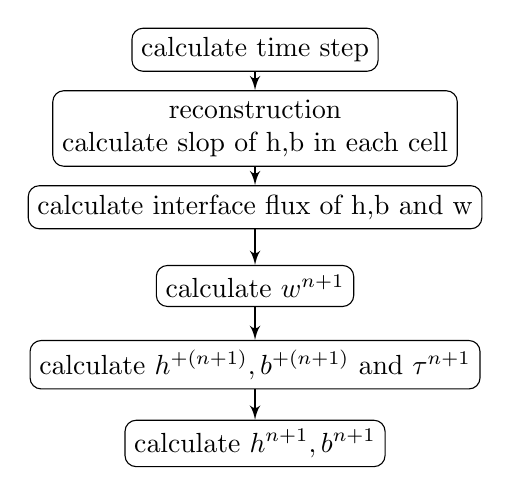
\begin{tikzpicture}[thick]
            \path[line] node[block] (time) {calculate time step};
            \path[line] node[block,below of=time] (interp) {reconstruction \\ calculate slop of h,b in each cell}
            (time) edge (interp);
            \path[line] node[block,below of=interp] (flux) {calculate interface flux of h,b and w}
            (interp) edge (flux);
            \path[line] node[block,below of=flux] (new-w) {calculate $w^{n+1}$}
            (flux) edge(new-w);
            \path[line] node[block,below of=new-w] (new-g) {calculate $h^{+(n+1)}, b^{+(n+1)}$ and $\tau^{n+1}$}
            (new-w) edge (new-g);
            \path[line] node[block,below of=new-g] (new-f) {calculate $h^{n+1}, b^{n+1}$}
            (new-g) edge (new-f);
        \end{tikzpicture}
    \end{center}
    \caption{solution algrithm in one iteration}
\end{figure}

\section{Nondimensionalization}
In the program, the following nondimensionalization is used,
\begin{gather*}
    \hat t=\frac{t}{t_\infty},\ \hat u_x=\frac{u_x}{C_\infty},\ \hat x=\frac{x}{L},\ \hat \rho=\frac{\rho}{\rho_\infty},\ \hat T=\frac{T}{T_\infty} \\
    \hat p=\frac{p}{\rho_\infty C_\infty^2},\ \hat q_i=\frac{q_i}{\rho_\infty C_\infty^3},\ \hat h=\frac{h}{\rho_\infty/C_\infty},\ \hat b=\frac{b}{\rho_\infty},\ \hat E=\frac{E}{C_\infty^2}
\end{gather*}

The free stream variables are related through
$$C_\infty=\sqrt{2RT_\infty},\ t_\infty=\frac{L}{C_\infty},\ \lambda_\infty=1/C_\infty^2$$

In the following, all variables are nondimensioned, but we will drop the \textasciicircum for simplicity. After nondimensionalization and using the reduced distribution function, the expressions for macroscopic variables become
\begin{equation} 
    \begin{aligned}
        &\rho=\int h{\rm du}=\sum\alpha_k h_k\\
        &\rho U=\int hu{\rm du}=\sum\alpha_k h_k u_k\\
        &\rho E=\frac{1}{2}\left(\int hu^2{\rm du}+\int b{\rm du}\right)=\frac{1}{2}\left(\sum\alpha_k h_k u_k^2+\sum\alpha_k b_k\right)
    \end{aligned}
\end{equation}
\begin{equation} 
    \frac{k+1}{2}p=\int(u-U)^2h{\rm du}+\int b{\rm du}=\sum\alpha_k(u_k-U)^2 h_k+\sum\alpha_k b_k
\end{equation}
\begin{equation} 
    \begin{aligned}
        q&=\frac{1}{2}\left[\int(u-U)(u-U)^2h{\rm du}+\int(u-U)b{\rm du}\right]\\
         &=\frac{1}{2}\left[\sum\alpha_k (u_k-U)(u_k-U)^2 h_k+\sum\alpha_k (u_k-U)b_k\right]
    \end{aligned}
\end{equation}
where $\alpha_k$ is the weight of the numerical integration at the k-th particle velocity. The summation is over all the discrete particle velocity.

The equation of state
\begin{equation} 
    p=\frac{1}{2}\rho T,\quad \lambda=\frac{1}{T}
\end{equation}

Other expressions are not changed.

\section{Time step and reconstruction}
The time step is determined by the CFL condition
\begin{equation} 
    \Delta t={\rm CFL}\frac{\Delta x}{|U|+c}
\end{equation}
where CFL is the CFL number, $c$ is the speed of sound. The macrocopic velocity $U$ can also be replace by $\max(U,u)$

In the program, the van Leer limiter is used for the reconstruction. For example, the slope of $h$ at the i-th cell and k-th particle velocity is
\begin{equation} 
    \sigma_{i,k}^h = ({\rm sign}(s_1)+{\rm sign}(s_2))\frac{|s_1||s_2|}{|s_1|+|s_2|}
\end{equation}
where $s_1=(h_{i,k}-h_{i-1,k})/(x_i-x_{i-1}), s_2=(h_{i+1,k}-h_{i,k})/(x_{i+1}-x_{i})$.

The slope of $b$ is calculated in the same way.

\section{Calculation of interface flux}
Take the interface $x_{i+1/2}=0$ at $t^n=0$ as example.

\subsection{The algrithm}
Here the original distribution function is used for illustration. From Eq. \ref{eq:csolution}, the integral solution at the cell interface is
\begin{equation}
    f(0,t,u_k,\xi)=\frac{1}{\tau}\int_{0}^t f^+(x',t',u_k,\xi)e^{-(t-t')/\tau}dt'+e^{-t/\tau}f_0(-u_kt,0,u_k,\xi)
\end{equation}

The initial distribution function $f_0$ is
\begin{equation}
    f_0(-u_kt,0,u_k,\xi) = 
    \begin{cases}
        f_{i+1/2,k}^L-\sigma_{i,k}u_kt,& u_k\geqslant 0\\ 
        f_{i+1/2,k}^R-\sigma_{i+1,k}u_kt,& u_k< 0\\ 
    \end{cases}
\end{equation}
where $f_{i+1/2,k}^L,f_{i+1/2,k}^R$ are obtained thourgh the reconstruction

The Maxwellian distribution in $f^+$ is approxmiated by
\begin{equation} 
    g(x,t,u,\xi)=g_0[1+(1-H[x])a^Lx+H[x]a^Rx+At]
\end{equation}
where $g_0$ is the Maxwellian distribution at $x=0,t=0$ and $H[x]$ is the Heaviside function$$H[x]=\begin{cases}0,& x<0\\ 1,& x\geqslant 0\end{cases}$$

%The slope $a^L,a^R$ can be calculated by the slope of conservative variables, and the slope $A$ is calculated by the compability condition

\subsection{The numerical procedure}
\section{Update cell averaged value}
\section{Boundary condition}

%usage
\chapter{Usage}
This chapter describes how to compile the source code and documentation.
Currently, it's only tested under Linux.
\section{Compile under *nix}
\section{Compile under windows}

%UGKS1D code
\chapter{UGKS1D Code}
This chapter describes the structure and the included shock structure test case at Ma=8.0 in the UGKS1D code.

%UGKS2D code
\chapter{UGKS2D Code}
This chapter describes the structure and the included lid-driven cavity test case in the UGKS2D code.
\section{test}
test

%license
\backmatter
\input{fdl}

%References
\cleardoublepage
\phantomsection
\addcontentsline{toc}{chapter}{Bibliography}
\bibliographystyle{unsrt}
\bibliography{manual}
\end{document}
